\begin{frame}
[plain]
  \titlepage
\end{frame}

\section{Введение}


\begin{frame}{Способы дизайна карманов связывания}
    \large
    \begin{itemize}
        %\setlength\itemsep{0.5cm}
        \item De novo
        \item “re-purposing”   
            \begin{itemize}
                \item  Направленная  эволюция
                \item Вычислительное моделирование
        \end{itemize}
    \end{itemize}
\end{frame}


\begin{frame}{Направленная эволюция}
\begin{itemize}
        \item Направленная эволюция - это общий термин
для описания набора методов молекулярной
биологии, которые, представляют собой
искусственный процесс мутирования и
отбора.
        \item Эти методы подразумевают собой случайное
(или направленное) внесение замен на
генетическом уровне с последующим
отбором белков, обладающих нужными
функциями.
\end{itemize}
\vspace{1cm}
Источник: http://dx.doi.org/10.4067/S0716-97602013000400011
\end{frame}


\begin{frame}{Вычислительное моделирование}
    Процесс дизайна белкового байндера посредством перепрофилирования
состоит из нескольких этапов:
    \begin{itemize}
        \item составление и курирование библиотеки белковых скаффолдов
        \item помещение лиганда в карман связывания
        \item  дизайн последовательности
        \item докинг лигандов + MD
        \item экспериментальная валидация результатов

    \end{itemize}

    Приведенная последовательность действий является только примером
организации вычислительного эксперимента, нежели строгим протоколом
\end{frame}


\begin{frame}{Составление и курирование библиотеки белковых
скаффолдов}
\includegraphics[width=0.9\textwidth]{scaffold-lib}
\end{frame}

\begin{frame}{Помещение лиганда в карман связывания. RosettaMatch}
    \includegraphics[width=0.9\textwidth]{rosetta-match}\\
    Источник: http://hdl.handle.net/1773/39951
\end{frame}

\begin{frame}{Дизайн последователþности, оптимизациā ротамеров}
    Используется алгоритм стохастического моделирования отжига
    (метод Моенте-Карло, имплементированнýй в Rosetta). Дизайн
    проводитсā при фиксированном белковом остове.
    Принцип работы в общем виде:
    \begin{itemize}
        \item  имеем начальный вид аминокислотного состава последовательности и ротамеров в окрестности кармана связявания
        \item  расчет энергии
        \item производится замена случайно выбранного остатка (точечная мутация)
        \item  расчет энергии,   если Enew < Eold то новый ротамер принимается, иначе ротамер принимается с некоторой вероятностю (к
    примеру, по критерию Метрополиса):
        \item  повторяем
    \end{itemize}
\end{frame}

\begin{frame}{Валидация}
\begin{itemize}
    \item Докинг можно использовать только с критическим анализом, из-за неподвижного остова белка
    \item Методы расширенной выборки в молекулярной динамики: метадинамика, awh ...
\end{itemize}
\includegraphics[width=0.9\textwidth]{funnel-metad}
\end{frame}
    

\begin{frame}{Примеры дизайнов. Дизайн байндера дигоксигенина (DIG)}
    Дигоксигенин (DIG) - агликон дигоксина, сердечного
    гликозида, который используется для лечения
    некоторых сердечно-сосудистых заболеваний
    \includegraphics[width=0.9\textwidth]{dig}
\end{frame}

\begin{frame}{Примеры дизайнов. Дизайн байндера дигоксигенина (DIG)}
       \includegraphics[width=0.8\textwidth]{dig-des}\\
       (a) Сайт связывания в DIG-связывающем липокаллине (Kd ~ 30.2 нМ, PDB: 1LKE)\\
(b) Cайт связывания анти-DIG антитела (Kd ~ 0.1 нМ, PDB: 1IGJ)\\
Источник: http://hdl.handle.net/1773/39951
\end{frame}


\begin{frame}{Дизайн белков, связывающих 17-ОПГ}
    17-ОПГ - 17-гидроксипрогестерон - гормон,
    производимый жёлтым телом яичников и корой
    надпочечников. Является биомаркером группы
    аутосомально-рецессивных заболеваний из группы
    "врожденная гиперплазия надпочечников"\\
    \includegraphics[width=0.8\textwidth]{17-opg}
\end{frame}
    
\begin{frame}{Дизайн белков, связывающих 17-ОПГ}
Для создания рабочей библиотеки скаффолдов
использовались NTF2-подобные белки из базы
данных PDB \\

В связи с тем, что 17-ОПГ имеет небольшое
количество полярных групп, авторы несколько
экспериментировали с вычислительными
подходами и первым делом определяли
комплементарность молекулярных форм лиганд -
белок (PathDock), а после искали водородные связи
с боковыми цепями аминокислот
\end{frame}

\begin{frame}{Дизайн белков, связывающих 17-ОПГ}
    \begin{itemize}
        \item Внимание авторов привлек резулþтат одного из дизайнов,
        белковой основой длā которого послужил белок с
        неизвестной функцией (RV0760) из
        Mycobacterium tuberculosis
        \item      По резулþтатам первой ÿксперименталþной проверки
        (метод дрожжевого дисплеā), ÿтот дизайн не смог свāзатþ
        17-ОПГ
    \end{itemize}
\end{frame}

\begin{frame}{Дизайн белков, связывающих 17-ОПГ}
    \begin{columns}
\begin{column}{0.5\textwidth}
    (a) взаимодействия в модели дизайна
    (b) взаимодействия в полученной
    структуре
    (c) структура 17-ОГП в модели дизайна
    показана фиолетовым, она
    сопоставлена со структурой 17-ОПГ из
    кристалла (цепь А, циан)
    (d) структуры 17-ОГП из кристалла -
    цепь А (циан), цепи B и D (маджента),
    цепь С (розовый)
    (e, f) лиганда в контексте белка
    Неудачный дизайн байндера 17-ОПГ
\end{column}
\begin{column}{0.5\textwidth}
    \includegraphics[height=0.7\textheight]{17-opg-des}
\end{column}
\end{columns}
\end{frame}
    
\begin{frame}{Дизайн de novo}
    В отличие от дизайна с перепрофилированием белковой функции, описанного
ранее, de novo дизайн в качестве входных данных не требует существования
предопределенного остова (из природного белка)\\

Сложности подхода:
    \begin{itemize}
        \item   сайты связывания малых молекул в однодоменных белках зачастую
        требуют наличия достаточно глубоких полостей, что опосредует
        нестабильность фолда
        \item для дизайна кармана связывания малых молекул требуется высокая
        точность определения нужной конформации остова и расположения
        боковых цепей
      \item  \*задача построения стабильного белкового скаффолда все еще остается
        нерешенной
    \end{itemize}
   
\end{frame}

\begin{frame}{Пример протокола de novo дизайна белков}
    \begin{itemize}
        \item   создание библиотеки белковых
        скаффолдов, собранных de novo из
        коротких пептидных фрагментов;
        \item   протокол лежит в открытом доступе
      помещение интересующей нас
        малой молекулы в заданный сайт
        связывания посредством
        алгоритма RIF
        (Rotamer-Interaction-Field)
        \item итеративная оптимизация
        последовательности и
        минимизация остова (Rozetta)
        \item   оптимизация взаиморасположения
        лиганда и окружающих его боковых   
        цепей аминокислот (увеличиваем    
        количество взаимодействий)
   \item  экспериментальная проверка   
    \end{itemize}
    Пример стратегии de novo дизайна белка-байндера,  источник: http://hdl.handle.net/1773/39951
\end{frame}


\begin{frame}{Пример алгоритма дизайна}
    “New computational protein design methods for de novo small molecule binding sites”\\
Источник: https://doi.org/10.1371/journal.pcbi.1008178\\
Авторы: James E. Lucas, Tanja Kortemme\\
Некоторые особенности метода:
\begin{itemize}
    \item   декомпозиция лиганда на подструктуры/фрагменты, для которых в PDB можно
    найти большое количество примеров взаимодействий.
    “Фрагмент” определяем как субструктуру молекулы-лиганда, представляющую
    собой самостоятельную химическую группу и состоящую как минимум из трех
    атомов;
    \item  делается предположение, что найденные контакты фрагмент - белок
    формируют пул возможных контактов целого лиганда с белком;
\end{itemize}
\end{frame}

\begin{frame}{Пример алгоритма дизайна. Декомпозиция лиганда}
    \includegraphics[width=0.8\textwidth]{lig-decompose}
\end{frame}    

\begin{frame}{Детали реализации}
    \begin{itemize}
        \item К каждому конформеру лиганда-мишени был применен алгоритм Монте-Карло - производилась
        сборка дискретных боковых цепей аминокислот из ансамбля контактов в композитный сайт
        связывания
        \item       
        Сайт связывания лиганда инициализировался тремя случайными остатками из ансамбля
        контактов
        \item
        Во время каждого шага алгоритма, боковая цепь случайного аминокислотного остатка в сайте
        связывания заменялась случайно выбранной боковой цепью из ансамбля контактов
        \item
        Вычислялся скор “нового” сайта связывания (энергия), шаг алгоритма принимался на основании
        критерия Метрополиса; цель - минимизация функции энергии
        \item
        Сайты связывания, характеризующиеся лучшими значениями энергии связывания
        релаксировались с использованием алгоритма FastRelax (Rosetta)
    \end{itemize}
   
\end{frame}

\begin{frame}{Inpainting}
    \centering
    \includegraphics[width=0.5\textwidth]{inpainting.png}
    \begin{itemize}
        \item Широкий спектр проблем проектирования структуры белков можно аналогичным образом сформулировать как проблемы восстановления недостающей информации 
        \end{itemize}

\end{frame}


\begin{frame}{Inpainting}
    \centering
    \includegraphics[width=0.8\textwidth]{halluc-inp.png}

\end{frame}

\begin{frame}{RFjoint}
    \centering
    \includegraphics[width=\textwidth]{rfjoint.png}
\end{frame}

\begin{frame}{"network hallucination"}
    \centering
    \includegraphics[width=\textwidth]{halluc}
\end{frame}

\begin{frame}{"network hallucination"}
    \centering
    \includegraphics[width=\textwidth]{halluc-mcmc}
\end{frame}


\begin{frame}{Ограниченные галлюцинации}
    \centering
    \includegraphics[width=0.5\textwidth]{halluc-motif}
    \begin{itemize}
        \item Cложная функцию потери, которая сочетает в себе часть из галлюцинаций с частью реконструкции мотива. 
        \item Подход с ограниченными галлюцинациями требует больших вычислительных ресурсов, поскольку для каждого шага градиентного спуска во время оптимизации последовательности требуется прямой и обратный проход через сеть.
        \end{itemize}
\end{frame}

\begin{frame}{Стратегии применеия ML моделей для дизайна карманов}
    \includegraphics[height=0.9\textheight]{binder-des-variants}    
\end{frame}

\begin{frame}{Диффузия}
    \centering
    \includegraphics[width=\textwidth]{diff-1}
\end{frame}

\begin{frame}{Диффузия}
    \centering
    \includegraphics[width=\textwidth]{diff-2}
\end{frame}

\begin{frame}{Диффузия}
    \centering
    \includegraphics[width=\textwidth]{diff-3}
     На каждом  шаге t модель берет X(t+1), а затем прогнозирует обновленную структуру X(0). Следующий ввод координат X(t-1) в модель генерируется
     путем интерполяции с шумом в направлении X(0).
\end{frame}

\begin{frame}{Partial Noise}
    \centering
    \includegraphics[width=0.8\textwidth]{partial-diff}\\
\end{frame}


\begin{frame}{Partial Noise, результаты}
    \centering
    \includegraphics[width=1\textwidth]{part-diff-results}\\
Высокая степень совпадения с AF2
\end{frame}

\begin{frame}{Дизайн по варианту укладки с AlphaFold}
    \centering
                \includegraphics[height=0.8\textheight]{alpha-design-1}  
\end{frame}

\begin{frame}{Дизайн по варианту укладки с AlphaFold}
    \centering
                \includegraphics[height=0.4\textheight]{alpha-design-2}  
\end{frame}

\begin{frame}{Частичный дизайн  с AlphaFold}
    \large
    \begin{itemize}
        \item Частичные галлюцинации
        \item Дизайн при заданном ходе остова
        \item "binder hallucination"
        \item Custom loss
    \end{itemize}
\end{frame}

\begin{frame}{MASIF}
    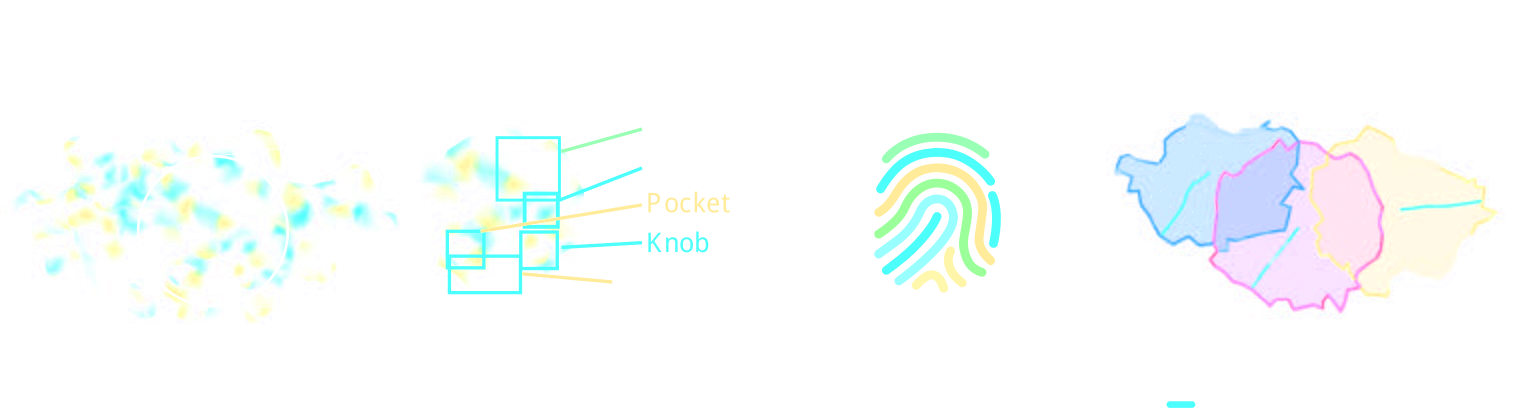
\includegraphics[width=.8\textwidth]{masif-1} \\
    MaSIF-site: классификатор, на входе  поверхность белка, на выходе  прогнозируемая оценка для каждой вершины поверхности на
вероятность участия в PPI
\end{frame}

\begin{frame}{MASIF, предсказание участков}
    \centering
    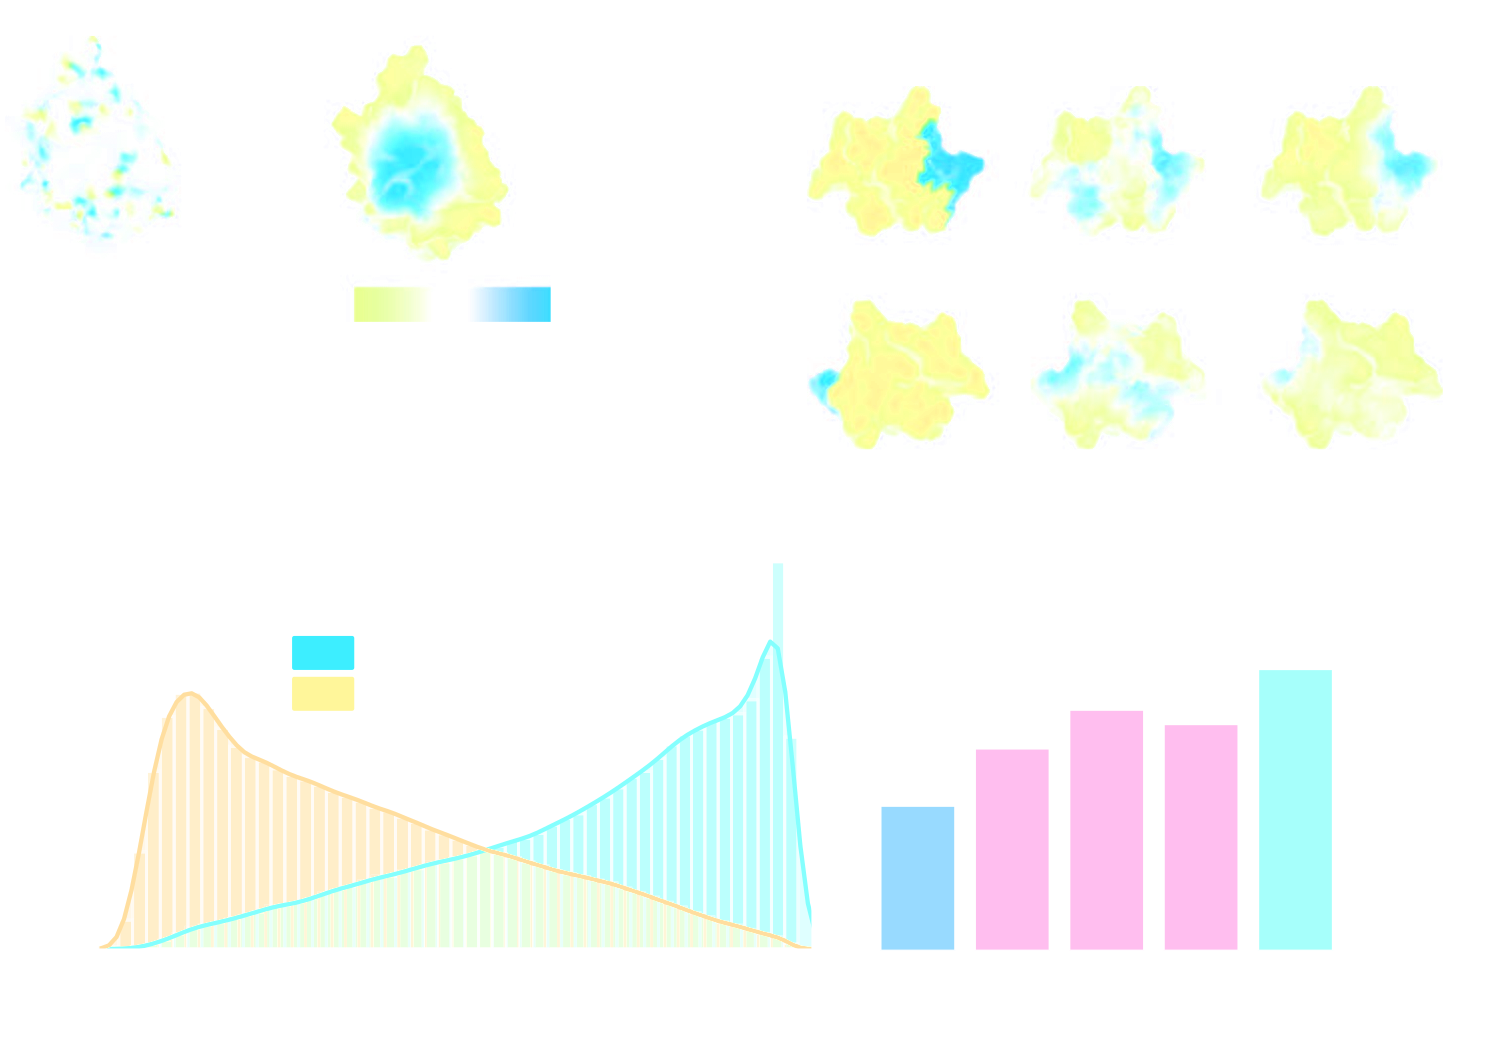
\includegraphics[width=.7\textwidth]{masif-ppi-1}

\end{frame}

\begin{frame}{Ultrafast scanning with MASIF}
    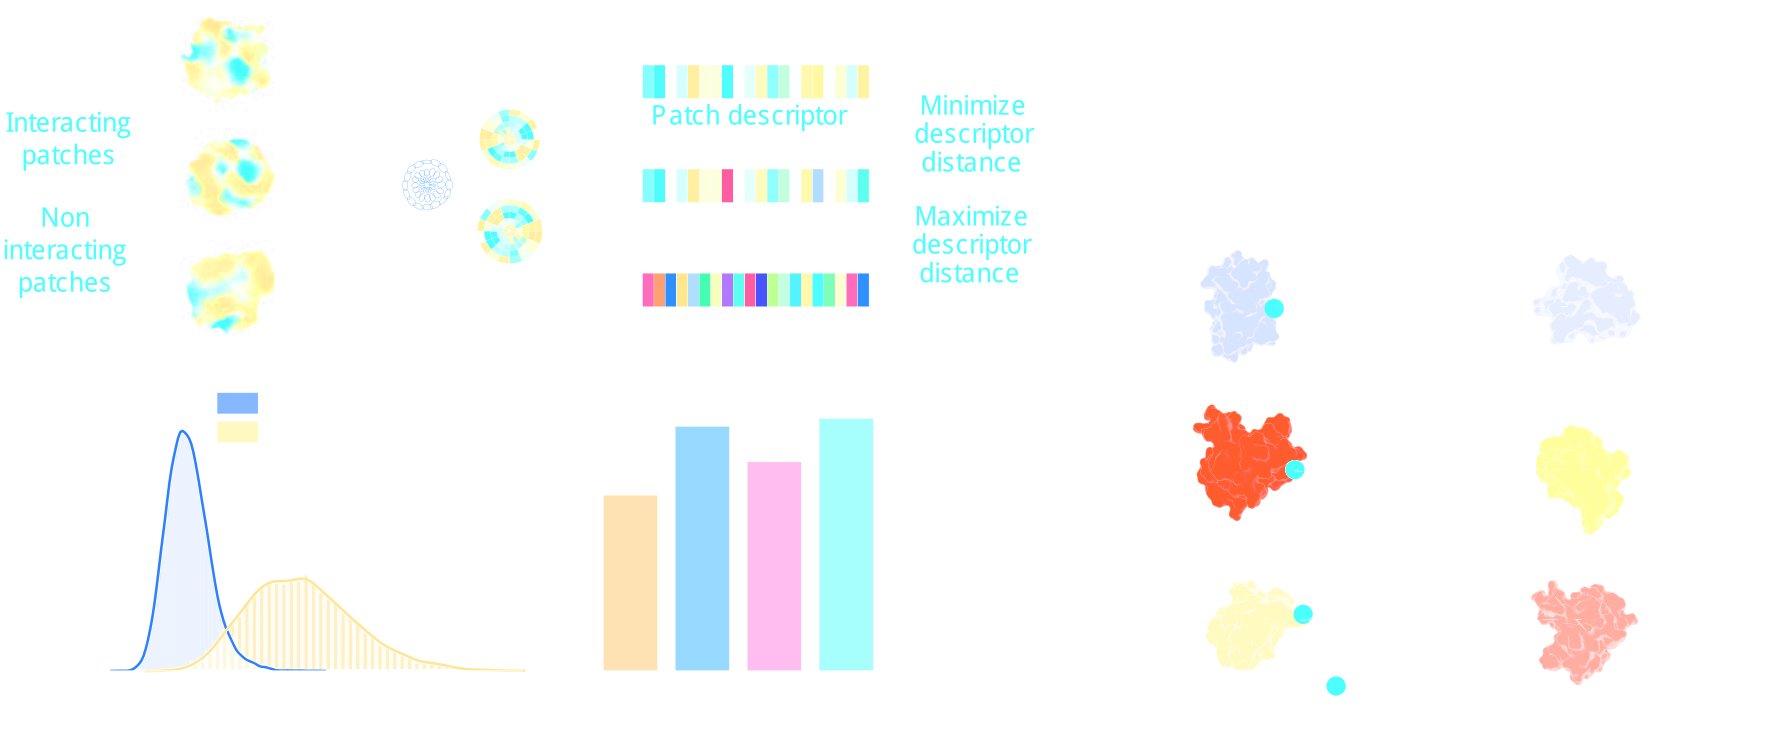
\includegraphics[width=.8\textwidth]{masif-ppi-scan}\\
    \footnotesize \*MaSIF-search inverts the numerical features of one  protein partner (multiplied by −1), with the exception of hydropathy. 
\end{frame}


\begin{frame}{Masif-seed}
    \centering
    \includegraphics[height=0.9\textheight]{masif-seed}  
\end{frame}




